\documentclass[journal]{IEEEtran}

\usepackage{amsmath,amssymb,amsfonts,mathtools}
\usepackage{bm}
\usepackage{graphicx}
\usepackage{booktabs}
\usepackage[nocompress]{cite}
\usepackage{algorithm}
\usepackage{algpseudocode}
\usepackage{multirow}
\usepackage{enumitem}
\usepackage{hyperref}

% Mathematical operators and symbols
\DeclareMathOperator{\sg}{sg}
\DeclareMathOperator{\clip}{clip}
\DeclareMathOperator{\softmax}{softmax}
\DeclareMathOperator{\PLPD}{PLPD}
\DeclareMathOperator{\RE}{RE}
\DeclareMathOperator{\ESS}{ESS}
\DeclareMathOperator{\RMS}{RMS}
\DeclareMathOperator*{\argmax}{arg\,max}

\begin{document}

\title{FedRAS: Continual Test-Time Adaptation of Federated Models via Reliability-Guided Adaptation and Sparse Restoration}

\author{
    \IEEEauthorblockN{Anonymous Authors}
}

\maketitle

\begin{abstract}
Continual test-time adaptation (CTTA) enables a deployed model to adapt to unlabeled and non-stationary test streams without accessing the original training data. However, continuous self-adaptation may progressively degrade a federated model after deployment, as unreliable target samples can introduce harmful updates and repeated adaptation can accumulate substantial parameter drift. Existing reliability-aware methods mainly regulate the current update, whereas restoration-based methods focus on limiting long-term drift, leaving these two problems insufficiently addressed together. In this paper, we propose FedRAS, a continual test-time adaptation approach for federated models via Reliability-Guided Adaptation (RGA) and Drift-Aware Sparse Restoration (DSR). RGA estimates sample reliability from complementary prediction and consistency cues to suppress unreliable contributions during online adaptation, while DSR periodically measures model displacement and selectively restores a small subset of parameters toward the federated anchor to limit accumulated drift without fully discarding useful adaptation. Extensive experiments under domain-wise and continual test-time adaptation settings demonstrate the effectiveness and robustness of FedRAS against representative adaptation methods.
\end{abstract}

\begin{IEEEkeywords}
Federated learning, continual test-time adaptation, sample reliability, sparse parameter restoration.
\end{IEEEkeywords}

\section{Introduction}
\label{sec:introduction}

Federated learning (FL) enables multiple clients to collaboratively train a shared model without transferring their raw data to a central server~\cite{1, 2}. After federated training, the resulting model is commonly deployed to edge devices and used independently of the training clients and server. However, the data encountered after deployment may differ substantially from the training distribution because of changing environments, sensing conditions, noise, blur, or other corruptions~\cite{3}. Continual test-time adaptation (CTTA) provides a practical way to address such distribution changes by continuously updating a deployed model using an unlabelled test stream while retaining the adapted state as the stream evolves~\cite{4, 5, 6}. Nevertheless, this continual self-adaptation also introduces a new risk: once an inappropriate update is incorporated into the model, its effect can be carried into subsequent predictions and updates, causing the deployed model to progressively deviate from its pre-deployment state.

Existing CTTA methods mainly improve adaptation from two complementary directions. Reliability-aware methods attempt to identify uncertain or unreliable target samples through entropy filtering, prediction consistency, perturbation responses, or related confidence measures, thereby reducing their influence on the current update~\cite{7, 8, 9}, while regional confidence further improves adaptation under complex shifts~\cite{10}. Although such strategies can suppress harmful gradients at individual adaptation steps, reliable or conservative updates do not necessarily guarantee long-term stability. Small parameter changes can still accumulate over a prolonged stream and gradually move the model away from its original representation. Another line of methods stabilizes continual adaptation through teacher models, memory mechanisms, regularization, or parameter restoration~\cite{11, 12, 13}. Recent advances also introduce confidence-gated selective parameter restoration~\cite{14}. These approaches can alleviate accumulated drift and preserve previously learned knowledge, but restoration alone does not determine which incoming samples should influence the preceding adaptation step. Moreover, overly aggressive restoration may erase parameters that remain useful for the current target distribution. Therefore, continuous test-time adaptation of a deployed federated model involves two related but distinct problems: unreliable target samples may produce harmful online updates, while repeated updates may accumulate into substantial parameter drift.

To address these two problems, two questions should be considered during continual adaptation. First, how can the influence of unreliable target samples be reduced before they induce harmful parameter updates? Prediction confidence alone may be insufficient because incorrect predictions can still be overconfident. Reliability should therefore be estimated from complementary evidence describing prediction certainty, structural sensitivity, decision confidence, agreement with the pre-deployment model, and prediction consistency under mild perturbations. Such reliability information can then be used to regulate how strongly each incoming sample participates in online adaptation. Second, how can accumulated parameter drift be controlled without discarding useful adaptation to the current target distribution? Completely resetting the adapted model to its initial state removes drift but simultaneously eliminates the knowledge acquired from the test stream. A more appropriate strategy is to monitor the displacement of the adapted parameters and selectively restore only a small subset of sufficiently displaced coordinates toward the original federated model. In this way, unreliable updates can be suppressed when they occur, while residual drift accumulated over repeated adaptation can be corrected afterwards.

Based on the above analysis, we propose \textbf{FedRAS}, a continual test-time adaptation approach for federated models via \textbf{Reliability-Guided Adaptation (RGA)} and \textbf{Drift-Aware Sparse Restoration (DSR)}. RGA evaluates each incoming target sample using complementary prediction and consistency cues and uses the resulting reliability to regulate sample contributions and the regional adaptation process. DSR periodically measures the displacement of the adapted model from the pre-deployment federated anchor, determines the amount of restoration according to the current adaptation state, and selectively pulls a small subset of normalization parameters toward their anchor values. The two components act at different stages of the same continual adaptation process: RGA reduces harmful updates before their effects accumulate, whereas DSR removes part of the parameter drift that remains after repeated online updates. The overall motivation and framework of FedRAS are illustrated in Figs.~\ref{fig:motivation} and~\ref{fig:framework}. The online procedure requires neither raw source samples nor further client--server communication after deployment.

The main contributions of this work are summarized as follows:
\begin{enumerate}[leftmargin=*]
    \item We formulate continual test-time adaptation of federated models from the joint perspective of unreliable online updates and accumulated parameter drift. Based on this observation, we introduce FedRAS, which combines reliability-guided adaptation with sparse parameter restoration under a source-free post-deployment setting without further client--server communication.
    \item We develop two complementary adaptation mechanisms to address these problems. RGA exploits multiple prediction and consistency cues to estimate target-sample reliability and regulate their contribution to online adaptation. DSR periodically monitors model displacement and selectively restores a small subset of adapted parameters toward the federated anchor, limiting accumulated drift without fully discarding useful target adaptation.
    \item We conduct extensive experiments under both independently reset corruption domains and uninterrupted continual test streams. The results demonstrate that FedRAS achieves strong continual adaptation performance while maintaining competitive retention on previously observed and clean distributions; controlled ablations further examine the contributions of reliability-guided adaptation and sparse restoration.
\end{enumerate}

\begin{figure*}[t]
\centering
\includegraphics[width=\textwidth]{F1.png}
\caption{Motivation for FedRAS. A deployed client receives the federated anchor $\theta_0$ and processes an unlabelled, non-stationary stream without raw source samples or further server communication. Standard CTTA may update on unreliable predictions and accumulate parameter drift. FedRAS coordinates reliability-guided updates with periodic sparse restoration toward $\theta_0$.}
\label{fig:motivation}
\end{figure*}

\section{Related Work}
\label{sec:related_work}

In this section, we review the research most closely related to FedRAS, including (1) federated learning and post-deployment adaptation; (2) test-time adaptation; (3) reliability-aware test-time adaptation; and (4) continual test-time adaptation and parameter restoration.

\subsection{Federated Learning and Post-Deployment Adaptation}
Federated learning (FL) enables multiple clients to collaboratively train a shared model without transmitting their raw data to a central server~\cite{1, 15}. Existing studies have extensively investigated optimization under heterogeneous client distributions, scalable coordination, and accelerated client gradients~\cite{16}. More recent studies have considered model adaptation after federated training. Test-time personalization adapts a trained federated model to individual clients using unlabeled target data, while related work has extended this idea to federated semantic segmentation and Bayesian prior-guided adaptation~\cite{17, 18, 19}, as well as prototype affinity topologies~\cite{20}. However, these approaches mainly focus on collaborative training or domain-specific adaptation, whereas the deployment setting considered in this work is more restrictive: after deployment, the client continuously receives a changing unlabeled stream without access to raw training samples or further client--server communication. FedRAS therefore focuses on maintaining effective adaptation of a federated model throughout a non-stationary post-deployment stream.

\subsection{Test-Time Adaptation}
Test-time adaptation (TTA) aims to adapt a pretrained model to unlabeled target data during inference without revisiting the original source training set~\cite{4, 25}. Tent performs lightweight adaptation by minimizing prediction entropy over BatchNorm affine parameters~\cite{4}. Subsequent approaches adapt classifier parameters, leverage curvature-aware zeroth-order optimization, or perform progressive embedding alignment to improve predictions without backpropagation overhead~\cite{21, 22, 23}. Compared with conventional source-free domain adaptation, TTA performs adaptation online as target samples arrive and is therefore particularly suitable for post-deployment distribution shifts. However, repeatedly updating the same model introduces additional risks when target distributions evolve over time. In such cases, the quality of each online update and the accumulation of parameter changes both become important for maintaining stable adaptation. FedRAS considers these two issues jointly in the continual deployment of federated models.

\subsection{Reliability-Aware Test-Time Adaptation}
Prediction entropy is widely used as an unsupervised signal for test-time adaptation, but low entropy does not necessarily imply a correct prediction. Consequently, several methods improve adaptation by explicitly estimating the reliability of incoming target samples. EATA filters high-entropy and redundant samples to reduce unreliable updates and catastrophic forgetting~\cite{7}. SAR combines reliable sample selection with sharpness-aware optimization to improve adaptation stability under dynamic test distributions~\cite{8}. DeYO evaluates prediction changes under patch shuffling to distinguish predictions that rely on meaningful spatial structure from those dominated by spurious cues~\cite{9}. ReCAP further measures confidence within regional perturbations and uses regional consistency to improve adaptation under challenging distribution shifts~\cite{10}. Dynamic reliability gating and ranked entropy minimization have also been explored to stabilize test-time optimization~\cite{24, 25}. Nevertheless, reliability-aware strategies primarily regulate which samples contribute to the current update and how strongly they influence optimization. They do not explicitly remove parameter drift that may accumulate after many individually reasonable adaptation steps. FedRAS therefore uses reliability information to regulate online adaptation while complementing it with a separate mechanism for controlling accumulated model drift.

\subsection{Continual Test-Time Adaptation and Parameter Restoration}
Continual test-time adaptation (CTTA) extends TTA to non-stationary streams in which the adapted model is retained as the test distribution evolves~\cite{5, 6}. Because each update affects subsequent predictions and adaptation steps, errors can accumulate over a long test stream. CoTTA stabilizes continual adaptation using a teacher model and stochastic parameter restoration~\cite{5}, while PeTTA addresses persistent adaptation under recurring distributions by maintaining adapted knowledge across repeated test scenarios~\cite{6}. Other CTTA methods employ memory banks and mean teachers~\cite{11, 12}, enforce topological consistency and dynamic memory coresets~\cite{26, 27}, or utilize complementary dual buffers~\cite{28} to reduce forgetting and stabilize long-term adaptation. Parameter restoration provides another direct strategy for limiting accumulated drift by moving selected model parameters toward their pre-adaptation values~\cite{13}. Recent work has further explored on-demand dynamic switching and structural alignment~\cite{29, 30}, as well as mixture-of-experts routing and neural collapse feature alignment~\cite{31, 32}. FedRAS differs by combining reliability-guided online adaptation with sparse parameter restoration, such that unreliable sample contributions are reduced during adaptation and accumulated parameter displacement is subsequently constrained.

\section{The Proposed FedRAS Method}
\label{sec:fedras_method}

\subsection{Problem Formulation and Notation}
Let $\theta_0 \in \mathbb{R}^d$ denote a pre-trained federated anchor model delivered to an edge client after decentralized training. Upon deployment, the client receives an unlabeled, non-stationary target stream $\mathcal{B} = \{B_t\}_{t=1}^T$, where each batch $B_t = \{x_i^t\}_{i=1}^{N_t}$ is drawn from time-varying distribution shifts. The online model is initialized as $\theta_1 = \theta_0$. Under the standard predict-then-update protocol, $B_t$ is first evaluated by the current state $\theta_t$ to produce predictions, after which the same batch is used to adapt the parameters to $\theta_{t+1}$. Crucially, the edge client operates in a source-free manner without raw training data or further server communication.

This continual deployment introduces two coupled challenges: (1) unlabeled target samples may provide noisy or misleading gradients that corrupt immediate updates; and (2) repeated online optimization inevitably accumulates residual parameter drift over long sequences, leading to severe representation decay. FedRAS tackles these challenges through synergistic sample-level reliability guidance and parameter-level sparse restoration.

\subsection{Overall Framework}
As illustrated in Fig.~\ref{fig:framework}, FedRAS coordinates two complementary modules: \textbf{Reliability-Guided Adaptation (RGA)} and \textbf{Drift-Aware Sparse Restoration (DSR)}. RGA operates on every incoming mini-batch to filter questionable samples and regulate their gradient contributions, while DSR runs periodically to detect accumulated parameter displacement and selectively contract key coordinates back toward the federated anchor.

\begin{figure*}[t]
\centering
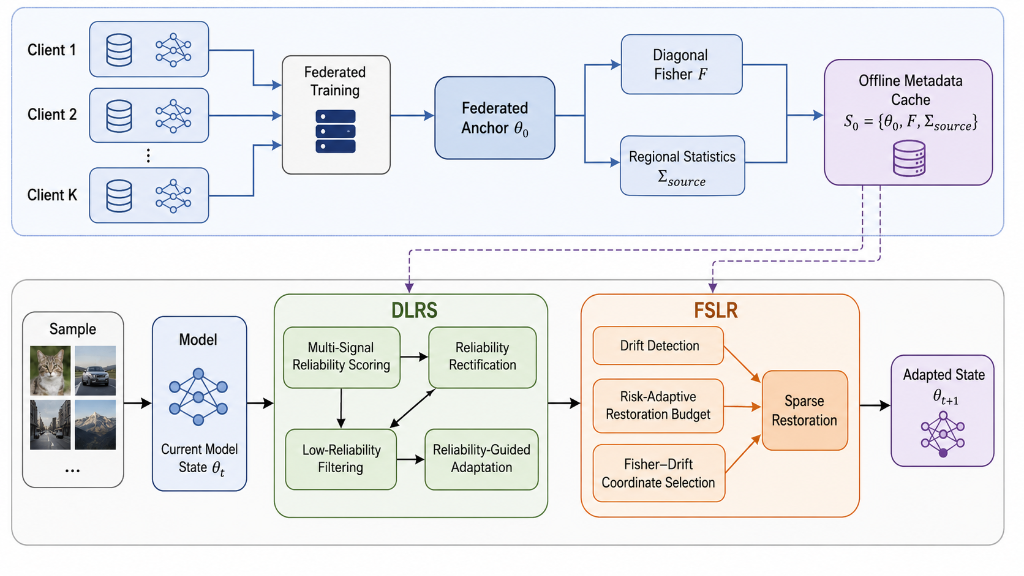
\includegraphics[width=\textwidth]{figures/fig2_framework.png}
\caption{Overall framework of FedRAS. Before deployment, federated training produces the anchor $\theta_0$ and a compact metadata cache. During deployment, RGA scores each target sample and performs a reliability-guided update. DSR then periodically measures drift, allocates a restoration budget, and pulls selected normalization coordinates toward $\theta_0$. Solid arrows denote online processing; dashed arrows denote access to cached metadata.}
\label{fig:framework}
\end{figure*}

\paragraph*{Cached Metadata and Trainable Scope}
Prior to deployment, the edge device caches a compact metadata footprint $\mathcal{S}_0 = \{\theta_0, \mathbf{F}, \Sigma_{\mathrm{src}}\}$. Here, $\mathbf{F} \in \mathbb{R}^{|\mathcal{A}|}$ is the diagonal Fisher information vector evaluated over the clean training data ($N_F = 50,000$ samples) at state $\theta_0$, where $F_j = \frac{1}{N_F} \sum_{i=1}^{N_F} (\frac{\partial \mathcal{L}_{\mathrm{ce}}}{\partial \theta_{0,j}})^2$ for each adaptable coordinate $j \in \mathcal{A}$, and $\Sigma_{\mathrm{src}}$ is the regional source feature covariance estimated from 500 clean instances. Following lightweight adaptation principles, the online trainable parameter scope $\mathcal{A}$ is strictly restricted to the affine scale ($\gamma$) and shift ($\beta$) parameters of BatchNorm layers in stages 1--3 of the ResNet-18 backbone~\cite{3} (totaling 4,480 scalar parameters, $<0.04\%$ of the network), while all convolution backbones and classifiers remain frozen.

Formally, for each incoming batch $B_t$, RGA first computes an intermediate adapted state $\theta_{t+\frac{1}{2}} = \mathcal{A}_{\mathrm{RGA}}(\theta_t, B_t; \mathcal{S}_0)$, after which DSR determines whether a restorative pullback is required. The unified online state transition is expressed as:
\begin{equation}
\label{eq:overall_transition}
\theta_{t+1} = \mathcal{R}_t \left[ \mathcal{A}_{\mathrm{RGA}}\left(\theta_t, B_t; \mathcal{S}_0\right) \right],
\end{equation}
where $\mathcal{R}_t$ represents the restoration operator, which reduces to the identity operator during non-restoration steps.

\subsection{Reliability-Guided Adaptation}
Because unsupervised objectives (e.g., entropy minimization) are vulnerable to overconfident erroneous predictions under severe corruptions, RGA evaluates target-sample reliability from multiple orthogonal cues and regulates both sample optimization weights and regional perturbation scales.

\subsubsection{Multi-Signal Reliability Estimation}
For each sample $x_i \in B_t$ with predicted class distribution $p_i = \softmax(f_{\theta_t}(x_i))$ and pseudo-label $\hat{y}_i = \argmax_c p_{i,c}$, RGA extracts three complementary confidence signals:
\begin{itemize}[leftmargin=*]
    \item \textbf{Predictive Certainty ($r_i^H$):} Derived from normalized Shannon entropy $H_i = -\sum_{c=1}^C p_{i,c} \log p_{i,c}$ as $r_i^H = \clip(1 - \frac{\sg[H_i]}{\log C}, 0, 1)$, where $\sg[\cdot]$ is the stop-gradient operator.
    \item \textbf{Patch-Shuffle Response ($r_i^P$):} Quantifies spatial-structural sensitivity by measuring the top-1 probability drop $\PLPD_i = \sg[p_{i,\hat{y}_i} - \tilde{p}_{i,\hat{y}_i}]$ after $4 \times 4$ grid patch shuffling~\cite{9}, defined as $r_i^P = \clip(\frac{\PLPD_i - \tau_P}{1 - \tau_P}, 0, 1)$ with threshold $\tau_P = 0.2$.
    \item \textbf{Decision Margin ($m_i$):} Captures boundary decisiveness via the gap between top-1 and top-2 probabilities $m_i = \sg[p_{i,(1)} - p_{i,(2)}]$.
\end{itemize}
These three cues are fused into a composite base reliability score:
\begin{equation}
\label{eq:base_reliability}
r_i^{(0)} = \sg\left[\clip\left(\alpha \frac{r_i^H + r_i^P}{2} + (1 - \alpha)m_i, 0, 1\right)\right],
\end{equation}
where $\alpha = 0.7$ balances structural certainty with decision margin.

\subsubsection{Reliability Rectification and Weighted Optimization}
To prevent self-reinforcing errors when the adapted model drifts, the base score $r_i^{(0)}$ is further rectified by frozen anchor verification and weak-view perturbation invariance:
\begin{equation}
\label{eq:final_reliability}
r_i = r_i^{(0)} (1 - \beta_a a_i) \left[\alpha_v + (1 - \alpha_v) e^{-J_i}\right] \cdot \mathbb{I}[r_i \ge \tau_H],
\end{equation}
where $a_i = \mathbb{I}[\argmax f_{\theta_t}(x_i) \neq \argmax f_{\theta_0}(x_i)]$ penalizes disagreement with anchor $\theta_0$ by factor $\beta_a = 0.3$, $J_i = D_{\mathrm{JS}}(p_i \parallel p_i^w)$ is the Jensen-Shannon divergence to a weakly perturbed view $x_i^w$ with consistency multiplier weight $\alpha_v = 0.8$, and $\tau_H = 0.2$ enforces a low-reliability truncation floor ($r_i \leftarrow 0$ if $r_i < \tau_H$).

The computed reliability $r_i$ dynamically scales the regional perturbation search radius $\eta_i = \eta_{\min} + (\eta_{\max} - \eta_{\min}) r_i \in [0.6, 1.2]$ and produces the joint product weight $w_i = \sg[r_i q_i]$, where $q_i = 2\sigma(\frac{0.7 \log C - \sg[\mathrm{RE}_i(\eta_i)]}{0.1 \log C})$ represents the regional confidence proxy~\cite{10}. The batch-normalized RGA objective is formulated as:
\begin{equation}
\label{eq:rga_loss}
\mathcal{L}_{\mathrm{RGA}} = \frac{\sum_{i \in B_t} w_i \mathrm{RE}_i(\eta_i)}{\max\left(\sum_{i \in B_t} w_i, \epsilon\right)}, \quad \epsilon = 10^{-12}.
\end{equation}
The intermediate state is updated via SGD with momentum $\mu = 0.9$ and learning rate $\eta_{\mathrm{lr}} = 10^{-3}$:
\begin{equation*}
v_{t+\frac{1}{2}, \mathcal{A}} = \mu v_{t, \mathcal{A}} + \nabla_{\theta_{\mathcal{A}}} \mathcal{L}_{\mathrm{RGA}}, \quad \theta_{t+\frac{1}{2}, \mathcal{A}} = \theta_{t, \mathcal{A}} - \eta_{\mathrm{lr}} v_{t+\frac{1}{2}, \mathcal{A}}.
\end{equation*}

\subsection{Drift-Aware Sparse Restoration}
While RGA suppresses unreliable updates per batch, residual parameter drift inevitably accumulates across prolonged non-stationary streams. Rather than blindly resetting all parameters, DSR periodically measures parameter displacement and adaptively pulls a sparse subset of critical coordinates back toward the federated anchor.

\subsubsection{Drift Detection and Risk-Adaptive Budget}
Every $R = 10$ batches ($t \bmod 10 = 0$), DSR evaluates the normalized parameter displacement $D_t = \frac{\|\theta_{t+1/2, \mathcal{A}} - \theta_{0, \mathcal{A}}\|_2}{\|\theta_{0, \mathcal{A}}\|_2 + \epsilon}$. The dynamic restoration budget fraction $\rho_t \in [0, 0.10]$ is determined jointly by batch adaptation risk and model displacement:
\begin{equation}
\label{eq:restoration_budget}
\rho_t = \rho_{\max} \cdot \clip(0.5 e_t + 0.5 a_t, 0, 1) \cdot \clip\left(\frac{D_t}{\tau_D}, 0, 1\right),
\end{equation}
where $\rho_{\max} = 0.10$, $\tau_D = 0.35$, $e_t = 1 - \frac{(\sum_i w_i)^2}{|B_t|(\sum_i w_i^2 + \epsilon)}$ is the effective sample size deficit, and $a_t = \frac{1}{|B_t|}\sum_{i \in B_t} a_i$ is the batch anchor disagreement rate. Thus, the restoration budget expands only when recent adaptation exhibits high uncertainty and significant drift.

\subsubsection{Fisher-Drift Coordinate Selection and Anchor Pullback}
Given the total coordinate budget $K_t = \lceil \rho_t |\mathcal{A}| \rceil$, DSR ranks candidate coordinates using layer-normalized Fisher-Drift sensitivity:
\begin{equation}
\label{eq:fisher_drift}
s_{t, \ell j} = \frac{F_{\ell j}}{\mathrm{RMS}(F_\ell) + \epsilon} \cdot \frac{|\theta_{t+\frac{1}{2}, \ell j} - \theta_{0, \ell j}|}{\mathrm{RMS}(d_{t, \ell}) + \epsilon},
\end{equation}
where $d_{t, \ell j} = |\theta_{t+1/2, \ell j} - \theta_{0, \ell j}|$. The budget $K_t$ is allocated across layers proportional to their positive score mass $M_{t, \ell} = \sum_j \max(s_{t, \ell j}, 0)$, subject to a per-layer cap $K_{t, \ell} \le 0.35 |\mathcal{A}_\ell|$. Within each layer $\ell$, the top-$K_{t, \ell}$ coordinates form the active restoration set $\mathcal{K}_t$.

For all selected coordinates $j \in \mathcal{K}_t$, DSR executes an elastic pullback toward $\theta_0$ with risk-adaptive strength $\lambda_t = 0.7(0.5 + 0.5 h_t d_t)$, and simultaneously resets their momentum buffers:
\begin{equation}
\label{eq:anchor_pullback}
\theta_{t+1, j} = \begin{cases} (1 - \lambda_t)\theta_{t+\frac{1}{2}, j} + \lambda_t \theta_{0, j}, & j \in \mathcal{K}_t, \\ \theta_{t+\frac{1}{2}, j}, & j \notin \mathcal{K}_t, \end{cases} \quad \text{with } v_{t+1, j} \leftarrow 0 \text{ for } j \in \mathcal{K}_t.
\end{equation}
Clearing the momentum buffer on restored coordinates is crucial to prevent subsequent SGD momentum from immediately reversing the restorative pullback.

\subsection{Theoretical Analysis of FedRAS}
We analyze the theoretical guarantees of RGA and DSR on the continual trajectory:

\paragraph*{Bounded Contribution of Unreliable Updates}
Let $\mathcal{E}_t \subseteq B_t$ denote the set of incorrectly predicted samples in batch $B_t$ and assume individual sample gradient norm is bounded by $\|g_i\|_2 \le G$. By the triangle inequality, the gradient contribution from erroneous samples satisfies:
\begin{equation}
\label{eq:grad_bound}
\left\| \frac{\sum_{i \in \mathcal{E}_t} w_i g_i}{\sum_{i \in B_t} w_i + \epsilon} \right\|_2 \le G \cdot \frac{\sum_{i \in \mathcal{E}_t} w_i}{\sum_{i \in B_t} w_i + \epsilon} = G \varepsilon_t^w,
\end{equation}
where $\varepsilon_t^w$ is the weighted error mass. Consequently, whenever RGA assigns lower weights to unreliable instances, it strictly tightens the worst-case gradient contamination on the model.

\paragraph*{Contraction Guarantee of Sparse Restoration}
Let $\delta = \theta_{t+\frac{1}{2}} - \theta_0$ denote parameter displacement prior to restoration. Applying Eq.~\eqref{eq:anchor_pullback} over the selected coordinates $\mathcal{K}_t$ and unselected complement $\mathcal{K}_t^c$ yields:
\begin{equation}
\label{eq:contraction}
\|\theta_{t+1} - \theta_0\|_2^2 = \|\theta_{t+\frac{1}{2}} - \theta_0\|_2^2 - \lambda_t(2 - \lambda_t) \|\delta_{\mathcal{K}_t}\|_2^2.
\end{equation}
For any $0 < \lambda_t \le 1$, the quantity $\lambda_t(2 - \lambda_t) > 0$, guaranteeing that each DSR step strictly contracts the adapted parameters toward the federated anchor space.

The complete online execution flow of FedRAS is summarized in Algorithm~\ref{alg:fedras}.

\begin{algorithm}[t]
\caption{FedRAS for Continual Test-Time Adaptation}
\label{alg:fedras}
\begin{algorithmic}[1]
\Require Federated anchor $\theta_0$; cached metadata $\mathcal{S}_0 = \{\theta_0, \mathbf{F}, \Sigma_{\mathrm{src}}\}$; target stream $\{B_t\}_{t=1}^T$.
\State Initialize $\theta_1 \gets \theta_0$ and momentum $v_1 \gets 0$.
\For{$t = 1, \dots, T$}
    \State Predict $B_t$ using $\theta_t$.
    \Statex \quad \textit{// Reliability-Guided Adaptation}
    \State Compute predictive certainty, patch response, and decision margin.
    \State Obtain base reliability $r_i^{(0)}$.
    \State Rectify reliability using anchor agreement and weak-view consistency.
    \State Set $r_i \gets 0$ for $r_i < \tau_H$.
    \State Determine regional scale $\eta_i$ and weight $w_i$.
    \State Update $\theta_t \to \theta_{t+\frac{1}{2}}$ using $\mathcal{L}_{\mathrm{RGA}}$.
    \Statex \quad \textit{// Drift-Aware Sparse Restoration}
    \If{$t \bmod R = 0$}
        \State Compute model displacement $D_t$.
        \State Compute batch risk $h_t$ and restoration fraction $\rho_t$.
        \State Determine sparse restoration set $\mathcal{K}_t$.
        \State Restore selected coordinates toward $\theta_0$.
        \State Clear momentum on restored coordinates.
    \Else
        \State $\theta_{t+1} \gets \theta_{t+\frac{1}{2}}$.
    \EndIf
\EndFor
\State \Return adapted model.
\end{algorithmic}
\end{algorithm}

\section{Experimental Evaluation}
\label{sec:experiments}

We conduct extensive experiments to evaluate FedRAS from three perspectives. First, we examine its adaptation performance under independently reset corruption domains. Second, we evaluate its long-term behavior under an uninterrupted continual test stream, where adaptation states are retained across distribution shifts. Third, we analyze the contributions of reliability-guided adaptation and sparse restoration through controlled ablations. All methods are initialized from the same federated model and follow the same predict-then-update evaluation protocol unless otherwise specified.

\subsection{Benchmark and Evaluation Protocols}

\subsubsection{Benchmark}
We primarily evaluate FedRAS on CIFAR-100 and its corrupted counterpart CIFAR-100-C~\cite{3}. CIFAR-100-C~\cite{3} contains 15 corruption types, and all corruptions are evaluated at severity level 5. Following the standard corruption taxonomy, the 15 corruptions are grouped into four categories: Noise, including Gaussian noise, shot noise, and impulse noise; Blur, including defocus blur, glass blur, motion blur, and zoom blur; Weather, including snow, frost, fog, and brightness; and Digital, including contrast, elastic transformation, pixelation, and JPEG compression. A ResNet-18 backbone~\cite{3} is used in the main experiments.

\subsubsection{Domain-Wise Adaptation Protocol}
We first evaluate the short-term adaptation capability of each method under independently reset corruption domains. For each corruption $c$, the model parameters and optimizer states are reset to the original federated anchor $\theta_0$ before processing the corresponding target stream. Therefore, adaptation within one corruption does not affect the evaluation of another corruption.

The overall domain-wise accuracy is defined as
\begin{equation}
A_{\mathrm{DW}} = \frac{1}{15} \sum_{c=1}^{15} A_c^{\mathrm{DW}},
\end{equation}
where $A_c^{\mathrm{DW}}$ denotes the prediction accuracy on corruption $c$. This protocol evaluates whether FedRAS remains competitive in conventional test-time adaptation when long-term cross-domain accumulation is removed.

\subsubsection{Continual Adaptation Protocol}
To evaluate long-term adaptation stability, we further construct an uninterrupted continual stream containing all 15 corruption domains. The model is initialized only once and sequentially processes the 15 corruptions for three complete cycles, resulting in a total of 45 corruption blocks. Neither the model parameters nor the optimizer state is reset during this process.

We report the average accuracy of the first and third cycles, denoted by $A_1$ and $A_3$, respectively. Continual performance change is measured by
\begin{equation}
\Delta_{3-1} = A_3 - A_1.
\end{equation}
A large negative $\Delta_{3-1}$ indicates performance deterioration during prolonged adaptation, whereas a value close to zero indicates stable continual behavior.

\subsubsection{Post-Adaptation Retention}
After completing the entire 45-block stream, online adaptation is disabled and the final model is frozen. We then evaluate it on clean CIFAR-100 and on the first four previously observed corruption domains. The former measures the retention of the pre-deployment representation, whereas the latter, denoted as Revisit, measures the ability to retain performance on previously encountered distributions after prolonged adaptation.

All reported results are the mean and sample standard deviation over three separately trained federated model instances.

\subsection{Comparison Methods}
We compare FedRAS with representative test-time and continual test-time adaptation methods. \textbf{Source} denotes the original federated model without test-time parameter updates. \textbf{Tent}, \textbf{EATA}, and \textbf{SAR} provide standard and reliability-aware test-time adaptation baselines. \textbf{RoTTA} and \textbf{PeTTA} are included as continual adaptation baselines. \textbf{DeYO~\cite{9}} and \textbf{ReCAP} provide additional comparisons based on patch-response reliability and regional confidence, respectively. We further include \textbf{ASR}, which provides a closely related restoration-oriented comparison.

All methods start from the same federated anchor and use the same predict-then-update timing without additional client-server communication during deployment.

\subsection{Implementation Details}
The main experiments use a batch size of 128 and SGD with a learning rate of $1.0 \times 10^{-3}$, momentum of 0.9, and zero weight decay. For RGA, the patch-shuffle operation uses a $4 \times 4$ grid. The patch-response threshold and multi-signal weighting coefficient are set to $\tau_P = 0.2$ and $\alpha = 0.7$, respectively. The regional perturbation scale varies between 0.6 and 1.2, and the low-reliability threshold is set to $\tau_H = 0.2$. Anchor-based rectification and weak-view consistency use $\beta_a = 0.3$ and $\alpha_v = 0.8$, respectively.

DSR is activated every $R = 10$ batches. The maximum restoration fraction is 0.10, while the normalized drift threshold and per-layer restoration cap are both set to 0.35. Gradients are clipped at a norm of 15.0. Diagonal Fisher statistics are computed from 50,000 labeled training samples, whereas the regional reference statistics are estimated from 500 clean samples.

During online adaptation, only 4,480 BatchNorm affine parameters are trainable, corresponding to less than 0.04\% of the complete network parameters. The remaining feature extractor and classifier parameters are frozen.

\subsection{Comparison With State-of-the-Art Methods}

\subsubsection{Domain-Wise Adaptation}
Table~\ref{tab:domain_wise} reports the domain-wise results under independent resets.

\begin{table*}[t]
\centering
\caption{Domain-wise results under independent resets on CIFAR-100-C~\cite{3} (severity 5). Mean $\pm$ std over three independent runs.}
\label{tab:domain_wise}
\begin{tabular}{lccccc}
\toprule
\textbf{Method} & \textbf{Noise} & \textbf{Blur} & \textbf{Weather} & \textbf{Digital} & \textbf{Overall Mean} \\
\midrule
Source & $19.5 \pm 0.9$ & $44.1 \pm 1.2$ & $54.1 \pm 0.5$ & $41.2 \pm 0.8$ & $41.0 \pm 0.5$ \\
Tent   & $\mathbf{54.7 \pm 0.7}$ & $\mathbf{64.3 \pm 0.1}$ & $64.9 \pm 0.2$ & $62.8 \pm 0.2$ & $62.2 \pm 0.1$ \\
EATA   & $49.3 \pm 1.2$ & $60.2 \pm 0.3$ & $60.9 \pm 0.1$ & $58.2 \pm 0.5$ & $57.7 \pm 0.2$ \\
SAR    & $53.7 \pm 0.6$ & $63.8 \pm 0.1$ & $64.2 \pm 0.3$ & $62.1 \pm 0.2$ & $61.4 \pm 0.1$ \\
ASR    & $\mathbf{54.7 \pm 0.7}$ & $64.2 \pm 0.1$ & $64.8 \pm 0.2$ & $62.8 \pm 0.2$ & $62.1 \pm 0.2$ \\
RoTTA  & $43.8 \pm 1.1$ & $58.7 \pm 0.3$ & $59.1 \pm 0.2$ & $53.4 \pm 0.3$ & $54.4 \pm 0.4$ \\
PeTTA  & $19.5 \pm 0.9$ & $44.1 \pm 1.2$ & $54.1 \pm 0.5$ & $41.2 \pm 0.8$ & $41.0 \pm 0.5$ \\
DeYO   & $54.1 \pm 0.4$ & $63.0 \pm 0.1$ & $63.9 \pm 0.1$ & $62.3 \pm 0.1$ & $61.5 \pm 0.2$ \\
ReCAP  & $54.1 \pm 0.3$ & $64.1 \pm 0.0$ & $64.9 \pm 0.3$ & $62.8 \pm 0.3$ & $62.0 \pm 0.2$ \\
\textbf{FedRAS} & $54.5 \pm 0.4$ & $\mathbf{64.3 \pm 0.1}$ & $\mathbf{65.2 \pm 0.3}$ & $\mathbf{63.1 \pm 0.3}$ & $\mathbf{62.3 \pm 0.2}$ \\
\bottomrule
\end{tabular}
\end{table*}

FedRAS achieves the highest overall domain-wise mean of 62.3\%, compared with 62.2\% for Tent, 62.1\% for ASR, and 62.0\% for ReCAP. The gain over the strongest competitors is modest, indicating that the principal advantage of FedRAS is not a large improvement under independently reset domains. More importantly, the result shows that introducing long-term restoration does not noticeably compromise the model's ability to adapt to an individual corruption domain.

Across corruption categories, FedRAS obtains the highest Weather and Digital averages and ties Tent for the highest Blur accuracy. Its Noise result is 0.2 percentage points below the best value obtained by Tent and ASR. These results suggest that FedRAS retains competitive short-term adaptation performance across different corruption families while introducing additional mechanisms for continual stability.

\subsubsection{Continual Adaptation and Retention}
Table~\ref{tab:continual} presents the more challenging continual evaluation, in which model and optimizer states are retained throughout all 45 corruption blocks.

\begin{table*}[t]
\centering
\caption{Continual evaluation across 3 cycles (45 blocks) and retention results on CIFAR-100-C~\cite{3}. Mean $\pm$ std over three runs.}
\label{tab:continual}
\begin{tabular}{lccccc}
\toprule
\textbf{Method} & \textbf{Cycle 1} & \textbf{Cycle 3} & $\bm{\Delta_{3-1}}$ & \textbf{Revisit} & \textbf{Clean} \\
\midrule
Source & $41.0 \pm 0.5$ & $41.0 \pm 0.5$ & $+0.0 \pm 0.0$ & $25.6 \pm 1.0$ & $\mathbf{77.0 \pm 0.2}$ \\
Tent   & $60.3 \pm 0.8$ & $27.3 \pm 2.5$ & $-33.0 \pm 3.3$ & $14.6 \pm 7.3$ & $19.3 \pm 8.3$ \\
EATA   & $57.1 \pm 0.2$ & $57.3 \pm 0.1$ & $+0.2 \pm 0.3$ & $52.3 \pm 0.8$ & $71.0 \pm 0.6$ \\
SAR    & $62.6 \pm 0.2$ & $62.3 \pm 0.3$ & $-0.3 \pm 0.2$ & $57.9 \pm 0.7$ & $72.4 \pm 0.8$ \\
ASR    & $63.4 \pm 0.2$ & $63.4 \pm 0.3$ & $+0.0 \pm 0.4$ & $\mathbf{58.8 \pm 0.0}$ & $74.1 \pm 0.3$ \\
RoTTA  & $54.7 \pm 0.4$ & $55.7 \pm 0.8$ & $+1.0 \pm 0.9$ & $41.6 \pm 2.5$ & $59.4 \pm 2.8$ \\
PeTTA  & $41.0 \pm 0.5$ & $41.0 \pm 0.5$ & $+0.0 \pm 0.0$ & $25.6 \pm 1.0$ & $74.1 \pm 0.2$ \\
DeYO   & $62.2 \pm 0.2$ & $60.7 \pm 0.5$ & $-1.5 \pm 0.3$ & $55.1 \pm 0.7$ & $68.8 \pm 0.7$ \\
ReCAP  & $62.5 \pm 0.3$ & $60.6 \pm 0.9$ & $-1.9 \pm 0.6$ & $55.1 \pm 0.6$ & $69.5 \pm 1.0$ \\
\textbf{FedRAS} & $\mathbf{63.5 \pm 0.2}$ & $\mathbf{63.7 \pm 0.1}$ & $+0.2 \pm 0.2$ & $58.0 \pm 0.3$ & $\mathbf{74.4 \pm 0.2}$ \\
\bottomrule
\end{tabular}
\end{table*}

The continual setting exposes a substantially different behavior from the independently reset evaluation. Tent initially improves the federated model to 60.3\% during Cycle 1 but subsequently drops to 27.3\% in Cycle 3, corresponding to a degradation of 33.0 percentage points. DeYO~\cite{9} and ReCAP are substantially more stable but still decrease by 1.5 and 1.9 percentage points, respectively. In contrast, FedRAS achieves 63.5\% in Cycle 1 and 63.7\% in Cycle 3, giving the highest Cycle-3 accuracy among the evaluated methods.

The post-stream evaluation further examines whether this continual performance is obtained at the expense of previously learned representations. FedRAS obtains a Revisit accuracy of 58.0\%, which is slightly below ASR at 58.8\%, while its Clean accuracy of 74.4\% is the highest among the adaptive methods. The unadapted Source model naturally retains the highest Clean accuracy because no target-domain updates are performed. Therefore, FedRAS should not be interpreted as being optimal on every retention metric. Instead, the results indicate that it provides the strongest final continual adaptation performance while maintaining a competitive level of post-adaptation retention.

These observations are consistent with the motivation of FedRAS: controlling unreliable updates is important for the current adaptation step, whereas periodic sparse restoration becomes particularly relevant when model states are inherited over a prolonged sequence.

\subsection{Generalization Evaluation}

\subsubsection{Evaluation on Tiny-ImageNet-C}
To investigate whether the effectiveness of FedRAS generalizes beyond CIFAR-100-C~\cite{3}, we further evaluate the compared methods on Tiny-ImageNet-C under the same domain-wise and continual adaptation protocols. The continual corruption ordering, number of cycles, restoration interval, and predict-then-update timing are kept consistent with the CIFAR-100-C~\cite{3} experiments unless otherwise specified.

\subsubsection{Generalization Across Backbones}
We additionally evaluate FedRAS with different network capacities to examine whether the proposed adaptation mechanism depends on a specific backbone. ResNet-18 and ResNet-34 are trained using the same federated learning protocol and subsequently evaluated under the same continual corruption stream.

\subsubsection{Different Federated Initializations}
The main experiments initialize all adaptation methods from FedACG~\cite{16}. To separate the contribution of continual adaptation from the quality of the federated initialization, we further evaluate FedRAS using models obtained from different federated training algorithms.

\subsection{Further Analysis}

\subsubsection{Component Ablation}
We evaluate the contributions of RGA and DSR separately and in combination. DSR provides the clearest independent contribution to long-term retention. Compared with the Base configuration, DSR alone increases Cycle-3 accuracy from 61.6\% to 62.9\%, improves $\Delta_{3-1}$ from $-1.5$ to $-0.3$ percentage points, and raises Clean accuracy from 70.4\% to 75.2\%. In contrast, RGA alone improves the continual degradation from $-1.5$ to $-1.1$ percentage points but does not independently increase Domain-wise or Cycle-3 accuracy.

When the complete configuration is used, FedRAS-Full achieves the strongest Cycle-1, Cycle-3, continual-change, and Revisit results among the evaluated variants. However, its Clean accuracy is slightly lower than FedRAS-Core. These results indicate that sparse restoration accounts for most of the measured retention improvement, whereas the contribution of RGA is more evident in the complete continual adaptation configuration than when it is used independently.

\subsubsection{Reliability-Weighting Formulation}
We next examine whether the particular formulation used to convert sample reliability into adaptation weights is itself responsible for the performance gain. To isolate this factor, the regional perturbation scale is fixed to $\eta = 1.2$, while the reliability threshold, anchor rectification, and weak-view consistency remain unchanged.

The controlled ablation shows that sample-only weighting provides higher Cycle-1, Cycle-3, Revisit, and Clean accuracy than product weighting, while regional-only weighting provides the smallest degradation between Cycles 1 and 3.

This result suggests that the benefit of FedRAS should not be attributed solely to the product weighting formulation. Rather, the final performance arises from the complete adaptation procedure, including reliability estimation, dynamic perturbation, and periodic restoration. The weighting formulation itself remains a design choice and is not uniformly optimal across all evaluation criteria.

\section{Conclusion}
\label{sec:conclusion}

In this paper, we investigated continual test-time adaptation for federated models under unlabeled and non-stationary deployment streams. We identified two key challenges in continuous self-adaptation: unreliable target samples may introduce harmful online updates, while repeated adaptation may gradually accumulate parameter drift. To address these problems, we proposed \textbf{FedRAS}, which integrates \textbf{Reliability-Guided Adaptation (RGA)} and \textbf{Drift-Aware Sparse Restoration (DSR)}. RGA estimates target-sample reliability from complementary prediction and consistency cues to regulate online adaptation, whereas DSR periodically detects accumulated model displacement and selectively restores a sparse subset of adapted parameters toward the federated anchor. Extensive experiments under both independently reset and continual corruption streams demonstrate that FedRAS maintains competitive short-term adaptation performance while improving long-term adaptation stability and representation retention. Ablation studies further show that sparse restoration provides the major contribution to long-term retention, while the complete FedRAS framework achieves the strongest overall continual adaptation performance among the evaluated configurations. Future work will investigate the applicability of FedRAS to larger-scale datasets, broader network architectures, and more diverse post-deployment distribution shifts.

\begin{thebibliography}{32}

\bibitem{1}
P.~Kairouz, H.~B.~McMahan, B.~Avent, A.~Bellet, M.~Bennis, A.~N.~Bhagoji, \emph{et~al.}, ``Advances and open problems in federated learning,'' \emph{Found. Trends Mach. Learn.}, vol.~14, no. 1--2, 2021.

\bibitem{2}
Y.~Wang, Z.~Chen, and X.~Liu, ``Federated continual test-time adaptation,'' \emph{IEEE Trans. Neural Netw. Learn. Syst.}, 2025.

\bibitem{3}
E.~Mintun, A.~Groner, V.~Kabra, D.~Spokoyny, S.~Kumar, and S.~Garg, ``On interaction between augmentations and corruptions in out-of-distribution robustness,'' in \emph{Adv. Neural Inf. Process. Syst. (NeurIPS)}, vol.~34, 2021.

\bibitem{4}
D.~Wang, E.~Shelhamer, S.~Liu, B.~Olshausen, and T.~Darrell, ``Tent: Fully test-time adaptation by entropy minimization,'' in \emph{Int. Conf. Learn. Represent. (ICLR)}, 2021.

\bibitem{5}
Q.~Wang, O.~Fink, L.~Van~Gool, and D.~Dai, ``Continual test-time domain adaptation,'' in \emph{Proc. IEEE/CVF Conf. Comput. Vis. Pattern Recognit. (CVPR)}, 2022.

\bibitem{6}
T.-H.~Hoang, D.~M.~Vo, and M.~N.~Do, ``Persistent test-time adaptation in recurring testing scenarios,'' in \emph{Adv. Neural Inf. Process. Syst. (NeurIPS)}, vol.~37, 2024.

\bibitem{7}
S.~Niu, J.~Wu, Y.~Zhang, Y.~Chen, S.~Zheng, P.~Zhao, and M.~Tan, ``Efficient test-time model adaptation without forgetting,'' in \emph{Proc. 39th Int. Conf. Mach. Learn. (ICML)}, vol. 162, 2022.

\bibitem{8}
S.~Niu, J.~Wu, Y.~Zhang, Z.~Wen, Y.~Chen, P.~Zhao, and M.~Tan, ``Towards stable test-time adaptation in dynamic wild world,'' in \emph{Int. Conf. Learn. Represent. (ICLR)}, 2023.

\bibitem{9}
J.~Lee, D.~Jung, S.~Lee, J.~Park, J.~Shin, U.~Hwang, and S.~Yoon, ``Entropy is not enough for test-time adaptation: From the perspective of disentangled factors,'' in \emph{Int. Conf. Learn. Represent. (ICLR)}, 2024.

\bibitem{10}
Z.~Hu, Y.~Hu, X.~Li, S.~Tang, and L.~Duan, ``Beyond entropy: Region confidence proxy for wild test-time adaptation,'' in \emph{Proc. 42nd Int. Conf. Mach. Learn. (ICML)}, 2025.

\bibitem{11}
T.~Gong, J.~Jeong, T.~Kim, Y.~Kim, J.~Shin, and S.-J.~Lee, ``NOTE: Robust continual test-time adaptation against temporal correlation,'' in \emph{Adv. Neural Inf. Process. Syst. (NeurIPS)}, vol.~35, 2022.

\bibitem{12}
M.~D{\"o}bler, R.~A.~Marsden, and B.~Yang, ``Robust mean teacher for continual and gradual test-time adaptation,'' in \emph{Proc. IEEE/CVF Conf. Comput. Vis. Pattern Recognit. (CVPR)}, 2023.

\bibitem{13}
T.~Lim, J.-W.~Hwang, and K.~Lee, ``When and where to reset matters for long-term test-time adaptation,'' in \emph{Int. Conf. Learn. Represent. (ICLR)}, 2026.

\bibitem{14}
X.~Zhang, C.~Yuan, and B.~Du, ``Selective parameter restoration and confidence gating for stable continual adaptation,'' in \emph{Proc. IEEE/CVF Conf. Comput. Vis. Pattern Recognit. (CVPR)}, 2026.

\bibitem{15}
X.~Li, M.~Jiang, X.~Zhang, M.~Kamp, and Q.~Dou, ``FedBN: Federated learning on non-IID features via local batch normalization,'' in \emph{Int. Conf. Learn. Represent. (ICLR)}, 2021.

\bibitem{16}
G.~Kim, J.~Kim, and B.~Han, ``Communication-efficient federated learning with accelerated client gradient,'' in \emph{Proc. IEEE/CVF Conf. Comput. Vis. Pattern Recognit. (CVPR)}, 2024.

\bibitem{17}
H.~Chen, Y.~Xu, Y.~Xu, Y.~Zhao, Y.~Zhang, and L.~Cui, ``Effective test-time personalization for federated semantic segmentation,'' \emph{Expert Syst. Appl.}, vol. 272, p. 126642, 2025.

\bibitem{18}
H.~Zhao, Y.~Ding, and X.~Tang, ``BPFedCTTA: Bayesian prior-guided federated continual test-time adaptation,'' in \emph{Proc. IEEE/CVF Conf. Comput. Vis. Pattern Recognit. (CVPR)}, 2026.

\bibitem{19}
Q.~Meng, W.~Dai, and J.~Chen, ``pFedBBN: Personalized federated test-time adaptation with balanced batch normalization,'' in \emph{Int. Conf. Learn. Represent. (ICLR)}, 2026.

\bibitem{20}
F.~Tan, L.~Zhao, and G.~Wang, ``Prototype affinity topology for federated continual test-time learning,'' in \emph{Proc. 43rd Int. Conf. Mach. Learn. (ICML)}, 2026.

\bibitem{21}
L.~Yang, X.~Gu, and H.~Dong, ``SNAP: Sparse test-time adaptation with low-latency updates in edge environments,'' in \emph{Adv. Neural Inf. Process. Syst. (NeurIPS)}, vol.~38, 2025.

\bibitem{22}
Y.~Liu, S.~Ren, and W.~Zhang, ``Curvature-aware zeroth-order optimization for memory-efficient test-time adaptation,'' in \emph{Proc. IEEE/CVF Conf. Comput. Vis. Pattern Recognit. (CVPR)}, 2026.

\bibitem{23}
B.~Wang, Q.~Shen, and J.~Xu, ``Progressive embedding alignment for backprop-free test-time adaptation,'' in \emph{Int. Conf. Learn. Represent. (ICLR)}, 2026.

\bibitem{24}
H.~Zhao, G.~Lin, and B.~Zhang, ``Entropy reliability scores and dynamic gating for wild test-time adaptation,'' in \emph{Adv. Neural Inf. Process. Syst. (NeurIPS)}, vol.~38, 2025.

\bibitem{25}
C.~Wang, Y.~Zhang, and J.~Sun, ``Ranked entropy minimization for robust test-time adaptation under dynamic shifts,'' in \emph{Proc. 42nd Int. Conf. Mach. Learn. (ICML)}, 2025.

\bibitem{26}
J.~Kim, H.~Park, and S.~Yoon, ``Topological consistency adaptation for continuous non-stationary test streams,'' in \emph{Proc. IEEE/CVF Conf. Comput. Vis. Pattern Recognit. (CVPR)}, 2025.

\bibitem{27}
D.~Feng, M.~Liu, and K.~Zhang, ``Dynamic prompt coreset and adaptive memory for continual test-time learning,'' in \emph{Proc. 42nd Int. Conf. Mach. Learn. (ICML)}, 2025.

\bibitem{28}
Y.~Chen, J.~Wu, and L.~Gao, ``CD-Buffer: Complementary dual-buffer adaptation for continual object recognition under adverse shifts,'' in \emph{Proc. IEEE/CVF Conf. Comput. Vis. Pattern Recognit. (CVPR)}, 2026.

\bibitem{29}
R.~Huang, P.~Wu, and Y.~Song, ``Hybrid-TTA: On-demand dynamic switching for test-time adaptation under compound corruptions,'' in \emph{Int. Conf. Learn. Represent. (ICLR)}, 2025.

\bibitem{30}
K.~Sun, M.~Zhang, and T.~Huang, ``SaTeen: Learning structural alignment for continual test-time adaptation,'' in \emph{Proc. 43rd Int. Conf. Mach. Learn. (ICML)}, 2026.

\bibitem{31}
W.~Zhou, H.~Li, and F.~Liu, ``TiME: Test-time mixture-of-experts routing for continual domain adaptation,'' in \emph{Proc. 43rd Int. Conf. Mach. Learn. (ICML)}, 2026.

\bibitem{32}
M.~Lin, S.~Wei, and Z.~Qian, ``Neural collapse feature-classifier alignment for unreliable pseudo-labels in continual TTA,'' in \emph{Proc. IEEE/CVF Conf. Comput. Vis. Pattern Recognit. (CVPR)}, 2026.

\end{thebibliography}

\end{document}